\section{Writing Algorithms in CCP}
\label{sec:ccp}
\begin{table}
    \centering
    \footnotesize
    \begin{tabular}{p{0.35\columnwidth}p{0.5\columnwidth}}
        \hline
        \hline
        \multicolumn{2}{c}{Primitive congestion signals} \\
        \hline
        \hline
        \textbf{Signal} & \textbf{Definition} \\
        \texttt{Ack.bytes\_acked}, \texttt{Ack.packets\_acked} & In-order acknowledged \\
        \texttt{Ack.bytes\_misordered}, \texttt{Ack.packets\_misordered} & Out-of-order acknowledged \\
        \texttt{Ack.ecn\_bytes}, \texttt{Ack.ecn\_packets} & ECN-marked \\
        \texttt{Ack.lost\_pkts\_sample} & Number of lost packets \\
        \texttt{Ack.now} & Datapath time (e.g., Linux \texttt{jiffies})\\
        \texttt{Flow.was\_timeout} & Did a timeout occur? \\
        \texttt{Flow.rtt\_sample\_us} & A recent sample RTT \\
        \texttt{Flow.rate\_outgoing} & Outgoing sending rate \\
        \texttt{Flow.rate\_incoming} & Receiver-side receiving rate  \\
        \texttt{Flow.bytes\_in\_flight}, \texttt{Flow.packets\_in\_flight} & Sent but not yet acknowledged \\
        & \\
        \hline
        \hline
        \multicolumn{2}{c}{Operators} \\
        \hline
        \hline
        \textbf{Class} & \textbf{Operations} \\
        Arithmetic & $+, -, *,$~/$,$ EWMA \\
        Assignment & $:=$ \\
        Comparison & $==, <, >$, or, and \\
        Conditionals & If (branching) \\
        & \\
        \hline
        \hline
        \multicolumn{2}{c}{Variable Scopes} \\
        \hline
        \hline
        \textbf{Scope} & \textbf{Description} \\
        \texttt{Ack} & Signals measured per packet \\
        \texttt{Flow} & Signals measured per connection \\
        %% \texttt{Control} & Never reset except by \texttt{update\_fields()} in user-space \\
        %% \texttt{Report} & Maintained until a call to \texttt{(report)}, then reset to defaults \\
        \texttt{Timer} & Multi-resolution timer that can be zeroed by a call to \ct{reset} \\
    \end{tabular}
    %\vspace{0.075in}
    \caption{Fast path language: primitive signals, operators, and scopes.}\label{tab:api}
\end{table}

Writing an algorithm in CCP involves specifying two callback functions,
\ct{onCreate()} and \ct{onReport()}, in the slow path (user-space). The slow path installs an
event-driven program in the fast path (kernel).
This ``split'' programming model involving both user and kernel mode allows
algorithms to perform computations flexibly in user-space, \eg compute a cubic
root, or use a machine learning algorithm to determine a sending rate, while
providing high performance by retaining frequently invoked logic within
the fast path.

Programs running in the fast path could compute summaries over per-packet
information (such as a minimum packet delay or a moving average of packet
delivery rate) and explicitly report summaries or high priority conditions
(such as loss) to the slow path component.

On a report from the fast path, the \ct{onReport()} handler in the slow path is
called, allowing the congestion control algorithm to set the flow's congestion
window or sending rate.
%
Meanwhile, the \ct{onCreate()} handler initializes a connection with a
fast path program and a default state.

\Para{Fast path programs.} CCP's fast path programs are written in a restrictive
domain-specific language.
%
For example, the following fast path program counts the cumulative
number of packets acknowledged and lost, while also reporting these counters to
the slow path immediately upon a loss:

{\footnotesize
\begin{minted}{lisp}
(def
    (acked 0)
    (lost  0))
(when true
    (:= acked (+ acked Ack.bytes_acked))
    (:= lost  (+ lost  Ack.lost_pkts_sample)))
    (fallthrough)
(when (> lost 0)
    (report))
\end{minted}
}

Conceptually, fast path programs contain state initializations, \ie a \ct{def}
clause, and event specifications, \ie a series of \ct{when} clauses.
%
The fast path checks event conditions on every packet acknowledgment and timeout.
%
If an event condition evaluates to true, \eg the number of lost packets is
nonzero, the body of the \ct{when} clause is executed as the corresponding
action.
%
For example, the \ct{report} instruction explicitly instructs the fast path to
transmit the \ct{acked} and \ct{lost} byte counters to the slow path whenever
the \ct{lost} counter becomes nonzero.
%
The summaries are reset to their initial values after every call to
\ct{report}.

Fast path programs have read access to {\em primitive congestion
  signals} (prefixed with ``\ct{Ack.}'' or ``\ct{Flow.}'' to specify their measurement period) that are
exposed by the kernel on every packet acknowledgment.
%
Such signals include statistics such as the round trip delay sample obtained
from the packet, the number of bytes that the stack believes have been dropped
by the network, the delivery rate of packets at the receiver, and so on.
%
The full list of primitive congestion signals is shown in Table~\ref{tab:api}.

\Para{Example: BBR.} As a more involved example, we show below
how various components of TCP BBR~\cite{bbr} are implemented using the CCP API.
%
A BBR sender estimates the rate of packets delivered to the receiver, and sets
its sending rate to the maximum delivered rate (over a sliding time
window), which is believed to the rate of the bottleneck link between the sender
and the receiver.

This filter over the received rate is expressed simply:
{\footnotesize
\begin{minted}{lisp}
(when true
    (:= minrtt
        (min minrtt Ack.rtt_sample_us))
    (:= curr_btl_est
        (max curr_btl_est Flow.rate_incoming))
    (fallthrough)
)
\end{minted}
}

Here, \texttt{(when true ...)} signifies that the body should be evaluated on every packet.
Correspondingly, \texttt{(fallthrough)} indicates that subsequent \texttt{when} clauses should be evaluated.

To determine whether a connection can send more than its current sending rate,
BBR probes for additional available bandwidth by temporarily increasing its
sending rate by a factor (1.25$\times$) of its current sending rate.
%
To drain a queue that may have been created in the process, it also reduces its
rate by a reciprocal factor (0.75$\times$) before starting to send at the new estimated
bottleneck link rate.

The following excerpt expresses this sending pattern (for simplicity, we show only 2 transitions):
{\footnotesize
\begin{minted}{lisp}
(when (== pulseState 0)
    (:= Rate (* 1.25 curr_btl_est))
    (:= pulseState 1))
(when (&& (== pulseState 1)
            (> Timer.micros Flow.rtt_sample_us))
    (:= Rate (* 0.75 curr_btl_est))
    (:= pulseState 2))
\end{minted}
}

Here, the variable \ct{pulseState} denotes the state of the sender's
bandwidth probing: probing with high sending rate (0) and draining queues with low
sending rate (1).
Each \texttt{when} clause represents a pulse state transition and is conditioned on the
resettable timer \texttt{Timer.micros}.
Upon the transition, the handler sets the \texttt{Rate} and advances \texttt{pulseState}.
After the last phase of the pulse, the handler would call \texttt{(reset)} to restart the sending pattern again (not shown).

Figure~\ref{fig:ccp:bbr} shows\footnote{We only show BBR's bandwidth and RTT probing (PROBE\_BW and PROBE\_RTT) phases here.}
the impact of BBR's bandwidth probing on the
achieved goodput and queueing delays when a single flow runs over a 96 Mbit/s
bottleneck link with a 100 ms round trip propagation delay.
%
BBR's windowed min/max operations and the RTT probing phase (showing steep rate
dips every 10 seconds) are implemented in the slow path's \ct{onReport()}
handler.
%
CCP's split programming model enables such flexible partitioning of
functionality, whereby complex operations and special cases can be implemented
in \userspace.

\Para{Slow path programs.} The \ct{onReport()} handler provides a way to
implement congestion control actions in \userspace.
If the round-trip time of the network is a few milliseconds or more,
it is possible to implement any congestion control algorithm completely in \userspace
with high fidelity relative to a per-packet update algorithm, as we show in \S\ref{sec:eval:fidelity}.
For example, a simple additive-increase
multiplicative-decrease (AIMD) algorithm could be implemented in Python\footnote{CCP's user-space component is implemented in Rust and exposes Python bindings.} using
the \ct{acked} and \ct{lost} bytes reported every round-trip time from the fast
path:

{\footnotesize
\begin{minted}{python}
def onReport(self, report):
  if report["lost"] > 0:
     self.cwnd = self.cwnd / 2
  else:
     acked = report["acked"]
     self.cwnd = self.cwnd + acked*MSS/self.cwnd
  self.update("cwnd", self.cwnd/MSS)
\end{minted}
}

We have implemented complex functionality within congestion control algorithms
by leveraging slow-path logic, for example, a congestion control
algorithm that uses signal processing techniques~\cite{nimbus}.

More broadly, developers may choose among various points in the algorithm design
space.
On one extreme, algorithms may be implemented almost entirely in \userspace,
using the fast path only as a queryable database of per-packet signals.
On the other extreme, CCP algorithms in \userspace may merely specify
transitions between fast path programs that implement the primary logic of the
algorithm.
Ultimately, users will partition algorithm functionality in the way
best suited to their performance requirements and choice of implementation complexity.

\begin{figure}[t]
\centering
    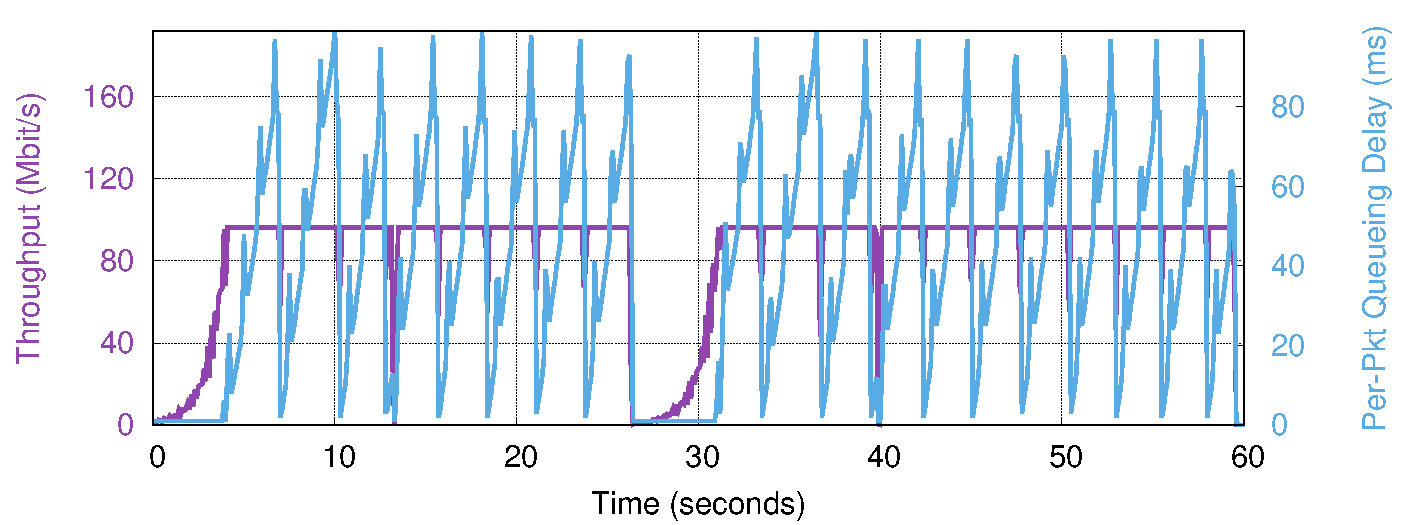
\includegraphics[width=\columnwidth]{img/bbr}
    \caption{
    Our CCP implementation of BBR used for a bulk transfer over a 96 Mbit/s link with a 100 ms RTT. The bandwidth probe phase can be seen in the oscillation of the queueing delay, and the RTT probe phase can be seen in the periodic dips in throughput.
    }\label{fig:ccp:bbr}
\end{figure}
